%\VignetteIndexEntry{Overview of the 'ddgraph' package}
%\VignetteKeywords{Graphical Modelling, Bayesian Networks}
%\VignettePackage{ddgraph}
\documentclass{article}
\usepackage[nogin]{Sweave}
\usepackage{hyperref}
\usepackage{cite}
\usepackage[authoryear,round]{natbib}
\usepackage{float}



\newcommand{\R}{\texttt{R} }
\newcommand{\Rfun}[1]{{\texttt{#1}}}
\newcommand{\Robj}[1]{{\texttt{#1}}}
\newcommand{\Rpackage}[1]{{\textit{#1}}}
\newcommand{\email}[1]{\href{mailto:#1}{\normalfont\texttt{#1}}}
%% colors
\usepackage{color}
\definecolor{Red}{rgb}{0.7,0,0}
\definecolor{Blue}{rgb}{0,0,0.8}

\hypersetup{%
  hyperindex = {true},
  colorlinks = {true},
  linktocpage = {true},
  plainpages = {false},
  linkcolor = {Blue},
  citecolor = {Blue},
  urlcolor = {Blue},
  pdfstartview = {Fit},
  pdfpagemode = {UseOutlines},
  pdfview = {XYZ null null null}
}

\author{Robert Stojni\'{c}\footnote{
  e-mail: \email{robert.stojnic@gmail.com},
  Cambridge Systems Biology Institute,
  University of Cambridge, UK}
}


\begin{document}

\title{Overview of the \Rpackage{ddgraph} package}

\maketitle

\tableofcontents

\section{Introduction}\label{sec:intro} 

This package implements the Neighbourhood Consistent PC Algorithm (NCPC) and Direct Dependence Graphs (DDGraphs) which show the dependence structure of a single target variable. 

The main goal of the NCPC algorithm is to infer direct from indirect dependencies to a target variable. Direct dependencies make up the causal neighbourhood of the target variable and in context of transcription binding profiles and gene regulation can be interpreted as the combinatorial code. This is achieved by performing conditional independence tests and therefore establishing statistical independence properties. NCPC has been shown to have a larger recall rate in scenarios with highly correlated variables (such as transcription factor binding profiles) which are weakly associated to a sparse target variable. For more details on the NCPC algorithm see \citep{stojnic_2012}. 

These methods are applicable to any data that come in a matrix format (both binary and continuous) as long as there is one biological target variable. The variables could for instance be either thresholded or threshold-free ChIP-chip/seq profiles, TF binding sites predictions, or indeed any set of biological features that are thought to influence (or are influenced by) a biological target variable. 

The package also implements a unified front-end to a number of other methods for inferring causal neighbourhood and Markov Blanket, as provided by packages \Rpackage{bnlearn} and \Rpackage{pcalg}. These methods include: Bayesian Network reconstruction using Hill-Climbing with BIC and BDe scores, IAMB, FastIAMB, InterIAMB, MMPC, MMHC with BIC/BDe scores and PC algorithm. 

The package is using the S4 class systems but with a limited number of generics. Accessors to data stored in S4 objects are implemented in more traditional list-like fashion using the \$ operator (similar to S3 and RefClass objects). 

\section{A toy example of finding the combinatorial code}

In this section we present a motivating example and explain the statistical and computational context for the NCPC algorithm. For more information about how to usage the package in a typical real-world application please skip to Section \ref{sec:case}.

Assume we are interested in finding transcription factors (TFs) that confer tissue-specificity to a set of cis-regulatory modules (CRMs), and we have the following datasets for a set of CRMs:

\begin{itemize}
\item A - a binary vector representing if transcription factor A binds to a CRM (e.g. obtained by thresholding a ChIP-chip signal)
\item B - a binary vector representing if transcription factor B binds to a CRM (e.g. obtained by thresholding a ChIP-chip signal)
\item T - a binary vector representing if a CRM is tissue specific (e.g. from transgenic reporter assays, proximity of tissue-specific genes, etc). 
\end{itemize}

This fictional dataset can be accessed with \Robj{data(toyExample)}. This is a \Robj{DDDataSet} object containing a data frame where columns are the two TFs and "class" representing the target variable T. See Section \ref{sec:create} on how to create a \Robj{DDDataSet} from a custom matrix. 


\begin{Schunk}
\begin{Sinput}
> library(ddgraph)
> data(toyExample)
> toyExample
\end{Sinput}
\begin{Soutput}
DDDataSet object: T 
with 200 data points of 2 variables with binary values
\end{Soutput}
\begin{Sinput}
> head(rawData(toyExample))
\end{Sinput}
\begin{Soutput}
  A B class
1 1 1     0
2 0 0     1
3 0 0     0
4 1 1     1
5 0 0     0
6 1 1     1
\end{Soutput}
\end{Schunk}

We are interested if A and/or B have a different binding pattern in those CRMs that are tissue specific (T=1) and those that are not (T=0). Traditionally, this is done by performing a Fisher's exact test. We would make a contingency table of T vs A, and T vs B and see if there is a statistical dependence between them. This gives us information about T-A and T-A independently of each other. We can do this with function \Rfun{ciTest}:

\begin{Schunk}
\begin{Sinput}
> ciTest(toyExample, "class", "A", test="fisher")
\end{Sinput}
\begin{Soutput}
Conditional independence test results using fisher 
  class[3] vs A[1], cond=[], reliable=TRUE, p.value=4.345314e-06
\end{Soutput}
\begin{Sinput}
> ciTest(toyExample, "class", "B", test="fisher")
\end{Sinput}
\begin{Soutput}
Conditional independence test results using fisher 
  class[3] vs B[2], cond=[], reliable=TRUE, p.value=0.0002472066
\end{Soutput}
\end{Schunk}

Both A and B show strong marginal dependence with the target variable (T internally represented as "class"), A more than B but both with fairly low P-values. Thus, both A and B are significantly associated with T. Next we might be interested in the combinatorial pattern of these two TFs. For instance, we might want to cluster our data (1 represented as black, and 0 as white):

\setkeys{Gin}{width=0.75\textwidth}
\begin{Schunk}
\begin{Sinput}
> heatmap(as.matrix(rawData(toyExample)), scale="none", col=c("white", "black"))
\end{Sinput}
\end{Schunk}
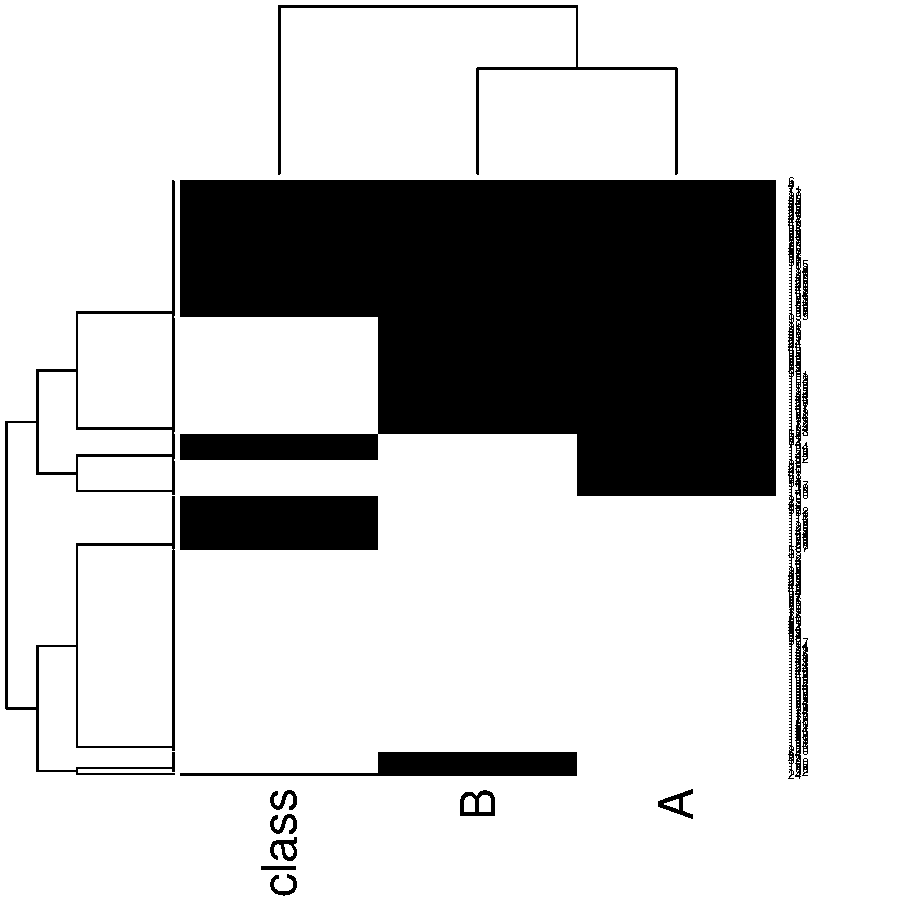
\includegraphics{ddgraph-cluster}

Visually we can see that there are clusters when A and B are bound where T=1 (top part of the diagram, T is represented with "class"), but we observe similar clusters for T=0 as well. Thus, it is unclear if there is any tissue-specific combinatorial pattern. 

The question if there is a tissue-specific combinatorial pattern can also be framed as: is T still dependent on B in the context of A? And vica versa, is T still dependent on A in the context of B. 

The question framed like this can be answered using a conditional independence test. This test is similar to marginal dependence test (e.g. Fisher's exact test), except that the data is grouped by one or more variables. If we suspect that A is a tissue-specific TF, and B not tissue specific then we would perform the T vs B test on two sub-datasets: one on CRMs where A=1 and one on CRMs where A=0. If the hypothesis is true, splitting the dataset by A should remove any dependence between T and B. 

Indeed, when we split the dataset by A, we find that in the two partitions (A=0 and A=1) there is no significant association between T and N (here represented as a single P-value):

\begin{Schunk}
\begin{Sinput}
> ciTest(toyExample, "class", "B", "A")
\end{Sinput}
\begin{Soutput}
Conditional independence test results using mc-x2-c 
  class[3] vs B[2], cond=A[1], reliable=TRUE, p.value=0.5804
\end{Soutput}
\end{Schunk}

Conversely, if we split the dataset by B, we still find significant association between T and A:

\begin{Schunk}
\begin{Sinput}
> ciTest(toyExample, "class", "A", "B")
\end{Sinput}
\begin{Soutput}
Conditional independence test results using mc-x2-c 
  class[3] vs A[1], cond=B[2], reliable=TRUE, p.value=0.0064
\end{Soutput}
\end{Schunk}

This suggests that A is directly associated with T ("class"), while B is associated only via its correlation with A. In terms of theory of causation, we say that A constitutes the causal neighbourhood of T.

Biologically this results suggests that A confers tissue-specificity, while B is associated with tissue-specific CRMs (T) via its correlation with A, possibly due to chromatin structure or other reasons independent of T. 

The NCPC algorithm works by running many such tests and contains additional checks for tests consistency which are especially important when the variables (in our case A and B) are highly correlated, which is the case for many TF binding profiles \citep{stojnic_2012}. 

Front-end function \Rfun{calcDependence()} will by default run the NCPC algorithm but can also run a number of other algorithms that infer the causal neighbourhood and the Markov Blanket.

\begin{Schunk}
\begin{Sinput}
> res <- calcDependence(toyExample)
> causalNeigh <- res$nbr
> causalNeigh
\end{Sinput}
\begin{Soutput}
[1] "A"
\end{Soutput}
\end{Schunk}
%$

The variables A, B and T need not to be binary. For instance, A and B could be raw ChIP-chip/seq signals over the CRMs, while T could be a probability of a CRM being tissue-specific. In that case, partial correlations would be used as a conditional independence test. That is, a linear relationship would be assumed between variables, and conditioning would be performed by building a regression model. 

\section{Case study - mesodermal CRMs in \textit{D. melanogaster}}\label{sec:case}

To demonstrate a typical pipeline we will use the example of mesodermal cis-regulatory modules (CRMs) in \textit{D. melanogaster} \citep{zinzen_combinatorial_2009}. This dataset comprises of genome-wide binding measurements (using ChIP-chip) for 5 transcription factors (TFs) at 1-5 time points. The binding sites were clustered into putative CRMs that were tested in transgenic reporter assays. 

In this section we assume that the user is familiar with the NCPC algorithm and the DDGraph visualisation vocabulary \citep{stojnic_2012}. 

\subsection{Example data}

The dataset is stored in a matrix format where rows are different observations (CRMs), while columns are different variables (TFs at time points). A column of name "class" is a reserved variable name for the target variable for which we are finding the causal neighbourhood and Markov Blanket. 


\begin{Schunk}
\begin{Sinput}
> library(ddgraph)
> data(mesoBin)
> names(mesoBin)
\end{Sinput}
\begin{Soutput}
[1] "neg"     "Meso"    "VM"      "SM"      "CM"      "Meso_SM"
[7] "VM_SM"  
\end{Soutput}
\begin{Sinput}
> head(rawData(mesoBin$VM))
\end{Sinput}
\begin{Soutput}
  Tin 2-4h Tin 4-6h Tin 6-8h Bin 6-8h Bin 8-10h Bin 10-12h Twi 2-4h
1        0        0        1        0         0          0        0
2        0        0        0        0         0          0        1
3        0        0        0        0         0          0        1
4        1        1        1        1         0          0        0
5        0        0        0        0         0          0        1
6        0        0        1        1         0          0        0
  Twi 4-6h Twi 6-8h Bap 6-8h Mef2 2-4h Mef2 4-6h Mef2 6-8h Mef2 8-10h
1        0        1        0         0         0         0          0
2        0        0        0         0         0         0          0
3        1        0        0         0         0         0          0
4        0        0        1         0         0         1          0
5        0        0        0         0         0         0          0
6        0        0        0         0         1         0          0
  Mef2 10-12h class
1           0     0
2           0     0
3           0     0
4           0     1
5           0     0
6           0     0
\end{Soutput}
\end{Schunk}
%$

The example dataset \Robj{mesoBin} is a list of \Robj{DDDataSet} objects, each corresponding to a different target CRM class. Each of the \Robj{DDDataSet} objects contains the binarized TF binding profiles. In the example above we show the binding profiles and target variable (CRM class membership) for the Visceral Muscle (VM) class of CRMs.

\subsection{Inferring direct from indirect dependencies}

The front-end function \Rfun{calcDependence()} calls various algorithm to infer the causal neighbourhood and Markov Blanket. 

\begin{Schunk}
\begin{Sinput}
> data(mesoBin)
> calcDependence(mesoBin$VM, "ncpc", verbose=FALSE)
\end{Sinput}
\begin{Soutput}
$obj
DDGraph produced with ncpc algorithm
Direct:  
Joint: Bin 6-8h Bin 8-10h 
Indirect: Tin 6-8h Bin 10-12h Twi 2-4h Twi 4-6h Bap 6-8h 
Using P-value alpha cutoff = 0.05 with conditional independence test = "mc-x2-c"

$nbr
[1] "Bin 6-8h"  "Bin 8-10h"

$labels
$labels$direct
NULL

$labels$joint
[1] "Bin 6-8h"  "Bin 8-10h"

$labels$indirect
[1] "Tin 6-8h"   "Bin 10-12h" "Twi 2-4h"   "Twi 4-6h"   "Bap 6-8h"  


$table
          name          type explained.by explained.pval
4     Bin 6-8h         joint    Bin 8-10h         0.0758
5    Bin 8-10h         joint     Bin 6-8h         0.0622
10    Bap 6-8h weak indirect     Bin 6-8h         0.0544
7     Twi 2-4h weak indirect     Bin 6-8h         0.1476
6   Bin 10-12h weak indirect    Bin 8-10h         1.0000
8     Twi 4-6h weak indirect    Bin 8-10h         0.1474
3     Tin 6-8h weak indirect     Bin 6-8h         0.6296
2     Tin 4-6h no dependence                          NA
9     Twi 6-8h no dependence                          NA
15 Mef2 10-12h no dependence                          NA
13   Mef2 6-8h no dependence                          NA
12   Mef2 4-6h no dependence                          NA
14  Mef2 8-10h no dependence                          NA
1     Tin 2-4h no dependence                          NA
11   Mef2 2-4h no dependence                          NA
   marginal.pval     log2FC
4         0.0006  1.9517448
5         0.0006  2.6147098
10        0.0064  1.6147098
7         0.0132 -1.7776076
6         0.0146  1.8211607
8         0.0216 -2.4441838
3         0.0316  1.1243842
2         0.3912  0.4627068
9         0.4170 -0.6416299
15        0.4662 -1.2921808
13        0.5696 -0.5729172
12        0.5832 -0.4002405
14        0.7396 -0.5816874
1         1.0000  0.1996723
11        1.0000 -0.5007674
\end{Soutput}
\begin{Sinput}
> calcDependence(mesoBin$VM, "hc-bic")
\end{Sinput}
\begin{Soutput}
$obj

  Bayesian network learned via Score-based methods

  model:
   [Tin 2-4h][Tin 4-6h|Tin 2-4h][Twi 4-6h|Tin 2-4h:Tin 4-6h]
   [Mef2 4-6h|Tin 4-6h:Twi 4-6h][Mef2 6-8h|Mef2 4-6h]
   [Tin 6-8h|Tin 4-6h:Mef2 6-8h][Twi 6-8h|Tin 4-6h:Mef2 6-8h]
   [Bap 6-8h|Tin 6-8h][Bin 6-8h|Bap 6-8h][Twi 2-4h|Twi 4-6h:Bap 6-8h]
   [Bin 8-10h|Bin 6-8h][Mef2 8-10h|Twi 2-4h:Mef2 6-8h]
   [Bin 10-12h|Bin 8-10h:Twi 2-4h][Mef2 10-12h|Mef2 4-6h:Mef2 8-10h]
   [target|Bin 8-10h][Mef2 2-4h|Tin 4-6h:Mef2 10-12h]
  nodes:                                 16 
  arcs:                                  24 
    undirected arcs:                     0 
    directed arcs:                       24 
  average markov blanket size:           3.75 
  average neighbourhood size:            3.00 
  average branching factor:              1.50 

  learning algorithm:                    Hill-Climbing 
  score:                                 
                                         Bayesian Information Criterion 
  penalization coefficient:              2.868286 
  tests used in the learning procedure:  480 
  optimized:                             TRUE 


$nbr
[1] "Bin 8-10h"

$mb
[1] "Bin 8-10h"
\end{Soutput}
\end{Schunk}

The result of \Rfun{calcDependence()} is a list of:
\begin{itemize}
\item \Robj{obj} - the resulting S3/S4 object depending on the method. This object can be used for plotting and obtain further information about the results.
\item \Robj{nbr} - the inferred causal neighbourhood of target variable
\item \Robj{mb} - the inferred Markov Blanket of target variable (if available for the method)
\item \Robj{labels} - a set of labels for the variables marking their dependence patterns (if available for the method)
\item \Robj{table} - a tabular representation of the results, sorted by P-value of marginal dependence (if available for the method). The "type" column represents the type of conditional independence pattern found. 
\end{itemize}

Each of the different algorithm take a number of parameters, e.g. the conditional independence test, P-value threshold, etc. For more information about these parameters consult the help page \Robj{?calcDependence}. 

\subsection{Direct Dependence Graphs}

The result of NCPC and NCPC* algorithm is a Direct Dependence Graph (DDGraph). The properties of this graph can be accessed using the \$ operator.

\begin{Schunk}
\begin{Sinput}
> data(mesoBin)
> res <- calcDependence(mesoBin$VM, "ncpc", verbose=FALSE)
> names(res)
\end{Sinput}
\begin{Soutput}
[1] "obj"    "nbr"    "labels" "table" 
\end{Soutput}
\begin{Sinput}
> dd <- res$obj
> class(dd)
\end{Sinput}
\begin{Soutput}
[1] "DDGraph"
attr(,"package")
[1] "ddgraph"
\end{Soutput}
\begin{Sinput}
> names(dd)
\end{Sinput}
\begin{Soutput}
 [1] "params"                       "final.calls"                 
 [3] "stats"                        "direct"                      
 [5] "joint"                        "indirect"                    
 [7] "conditional"                  "conditionalJoint"            
 [9] "directAndJoint"               "directAndJointAndConditional"
\end{Soutput}
\begin{Sinput}
> dd$params
\end{Sinput}
\begin{Soutput}
$alpha
[1] 0.05

$p.value.adjust.method
[1] "none"

$test.type
[1] "mc-x2-c"

$mc.replicates
[1] 5000

$verbose
[1] FALSE

$star
[1] FALSE

$min.table.size
[1] 10

$max.set.size
[1] 2
\end{Soutput}
\begin{Sinput}
> dd$joint
\end{Sinput}
\begin{Soutput}
 Bin 6-8h Bin 8-10h 
        4         5 
\end{Soutput}
\end{Schunk}
%$

For the VM CRM class we identified two variables: Bin 6-8h and Bin 8-10h as having the joint dependence pattern. To further explore this results we can plot the DDGraph that summarizes the conditional independence tests that lead to this result. P-values of conditional independencies are given on top of each edge. 

The DDGraph can be plotted by calling the \Rfun{plot()} function. The extra \Robj{col=TRUE} specifies to colour-code the node according to marginal enrichment (red) or depletion (blue). For more options see help page for \Robj{?plot}. 

\setkeys{Gin}{width=0.75\textwidth}
\begin{Schunk}
\begin{Sinput}
> plot(dd, col=TRUE)
\end{Sinput}
\end{Schunk}
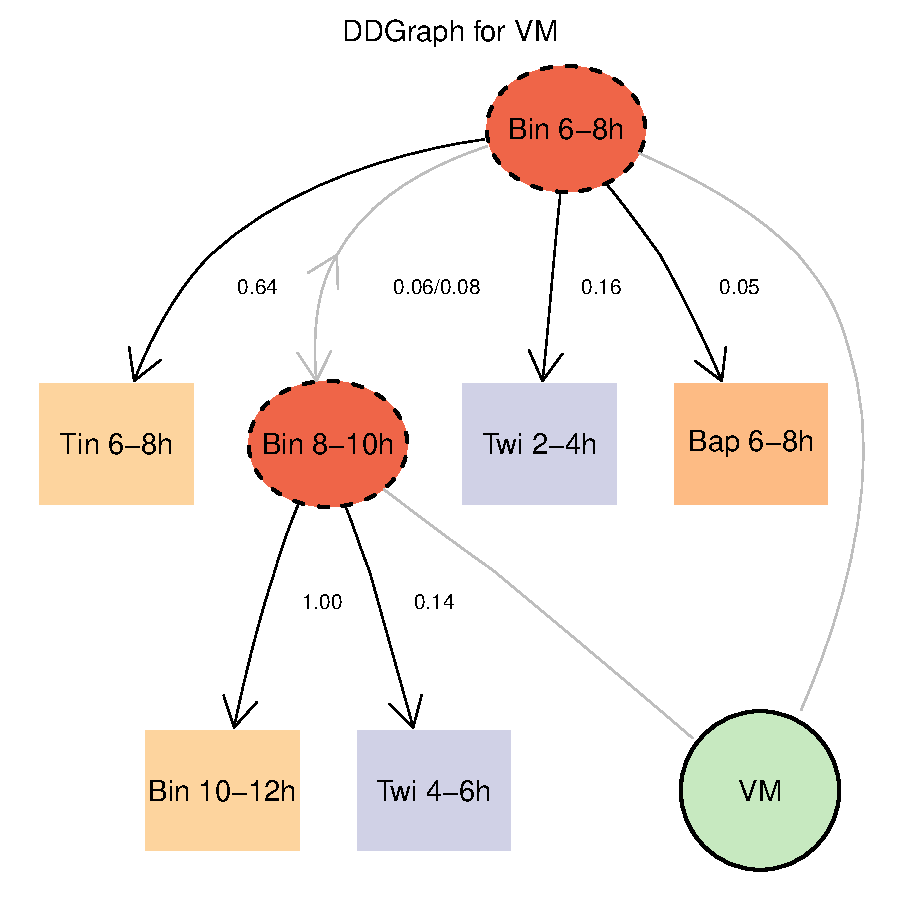
\includegraphics{ddgraph-ddgraph-plot}

\subsection{Testing combinations of values}

Once we identified Bin 6-8h and Bin 8-10h as candidates for the causal neighbourhood, we can examine which combinations of their values show most pronounced differences between the CRMs in the VM class, and the rest of CRMs. For binary data this can be achieved using the \Rfun{combinationsTest()} function. 

\begin{Schunk}
\begin{Sinput}
> combinationsTest(mesoBin$VM, c("Bin 6-8h", "Bin 8-10h"), 
+ 	p.adjust.method="fdr", verbose=FALSE)
\end{Sinput}
\begin{Soutput}
  combination      p.value freq.pos freq.neg     type fold.difference
1          00 0.0009870705        7      251 depleted            1.95
4          11 0.0021694910        5       13 enriched            7.07
3          10 0.2216949488        3       25 enriched            2.21
2          01 0.2743017082        1        5 enriched            3.67
\end{Soutput}
\end{Schunk}
%$

The output contains P-values adjusted using the Benjamini-Hochberg method for controlling false discovery rate, and is sorted in ascending P-value order. 

\subsection{Creating a new dataset}\label{sec:create}

A dataset can be created from scratch by invoking the function \Rfun{makeDDDataSet()}. The input is a matrix with rows as observations, columns as variables and the corresponding target variable. Only one target variable can be specified. Currently only binary and continuous data types are supported. 

\begin{Schunk}
\begin{Sinput}
> data <- matrix(rbinom(50, 1, 0.5), ncol=5)
> target <- c(0, 0, 0, 0, 0, 1, 1, 1, 1, 1)
> d <- makeDDDataSet(data, name="example data", classLabels=target)
> d
\end{Sinput}
\begin{Soutput}
DDDataSet object: example data 
with 10 data points of 5 variables with binary values
\end{Soutput}
\begin{Sinput}
> rawData(d)
\end{Sinput}
\begin{Soutput}
   V1 V2 V3 V4 V5 class
1   1  0  1  0  0     0
2   1  0  1  1  0     0
3   0  0  0  0  0     0
4   0  1  0  0  0     0
5   1  0  1  0  0     0
6   1  0  1  1  0     1
7   0  1  1  1  1     1
8   1  1  1  1  1     1
9   1  0  0  0  1     1
10  0  1  0  1  1     1
\end{Soutput}
\begin{Sinput}
> names(d)
\end{Sinput}
\begin{Soutput}
[1] "V1"    "V2"    "V3"    "V4"    "V5"    "class"
\end{Soutput}
\begin{Sinput}
> d$V1
\end{Sinput}
\begin{Soutput}
 [1] 1 1 0 0 1 1 0 1 1 0
\end{Soutput}
\begin{Sinput}
> d$class
\end{Sinput}
\begin{Soutput}
 [1] 0 0 0 0 0 1 1 1 1 1
\end{Soutput}
\end{Schunk}

If the data is already stored in an S4 object, we recommend implementing the \Rfun{toDDDataSet()} generic to provide a unified mechanism for obtaining \Robj{DDDataSet} instances.  

\section{Session info}

\begin{itemize}\raggedright
  \item R version 2.15.0 (2012-03-30), \verb|x86_64-pc-linux-gnu|
  \item Locale: \verb|LC_CTYPE=en_GB.UTF-8|, \verb|LC_NUMERIC=C|, \verb|LC_TIME=en_GB.UTF-8|, \verb|LC_COLLATE=C|, \verb|LC_MONETARY=en_GB.UTF-8|, \verb|LC_MESSAGES=en_GB.UTF-8|, \verb|LC_PAPER=C|, \verb|LC_NAME=C|, \verb|LC_ADDRESS=C|, \verb|LC_TELEPHONE=C|, \verb|LC_MEASUREMENT=en_GB.UTF-8|, \verb|LC_IDENTIFICATION=C|
  \item Base packages: base, datasets, grDevices, graphics,
    grid, methods, stats, utils
  \item Other packages: Rcpp~0.9.10, Rgraphviz~1.34.0,
    ddgraph~1.0.1, graph~1.34.0
  \item Loaded via a namespace (and not attached):
    BiocGenerics~0.2.0, MASS~7.3-16, RBGL~1.32.0,
    RColorBrewer~1.0-5, bnlearn~2.9, ggm~1.99-2, gtools~2.6.2,
    infotheo~1.1.0, pcalg~1.1-4, plotrix~3.4,
    robustbase~0.8-1-1, stats4~2.15.0, tools~2.15.0
\end{itemize}
\bibliographystyle{apalike}
\bibliography{references}

\end{document}ll
